\documentclass{ximera}

\begin{document}

\begin{question}
  Find 
  \[
  \displaystyle \lim_{x\to 2} \frac{x^2+7x+10}{x^2-4x+4}
  \]
  \begin{solution}
    \begin{hint}
     This function is \underline{not} continuous everywhere, but both the numerator and denominator are continuous everywhere as functions. Thus, if the limit of $\frac{x^2+7x+10}{x^2-4x+4}$ as $x\to{a}$ does not exist, then the denominator $x^2-4x+4$ must be zero at $a$. Does $x^2-4x+4=0$ when $x=2$? Does $x^2+7x+10=0$ at $x=2$ as well?
    \end{hint}
     \begin{hint}
    	Take a look at the graph of the function
    \begin{center}
     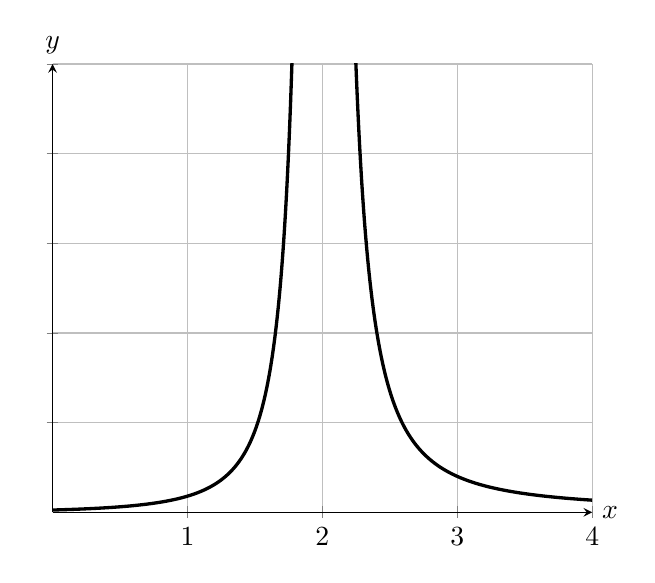
\begin{tikzpicture}
	\begin{axis}
	[ymin=0,ymax=500, axis lines=center,xlabel=$x$,ylabel=$y$,every axis y 
	label/.style={at=(current axis.above origin),anchor=south},every axis x label/.style={at=(current axis.right of origin),anchor=west},
	domain=0:4,
	yticklabels={},
	ymajorgrids=true,
	grid = major
	]
	\addplot[domain=0:197/100,very thick,smooth,samples=600]
	{(\x^2+7*\x+10)/(\x^2-4*\x+4)};
	\addplot[domain=203/100:4,very thick,smooth,samples=600]
	{(\x^2+7*\x+10)/(\x^2-4*\x+4)};
	\end{axis}
       \end{tikzpicture}      
      \end{center} 
    \end{hint}
    \begin{hint}
     Evaluating $\lim\limits_{x\to2}\frac{x^2+7x+10}{x^2-4x+4}$ we see that it tends to $\infty$. This follows because, for $x$, $x^2-4x+4\ge0$, and for $x\ge-2$, $x^2+7x+10\ge0$; hence, for $x\ge-2$, $\frac{x^2+7x+10}{x^2-4x+4}\ge0$. Moreover, $x^2-4x+4$ tends to $0$ as $x\to{2}$ and $x^2+7x+10$ tends to $28$ as $x\to{0}$. These two observations tell us that  $\lim\limits_{x\to2}\frac{x^2+7x+10}{x^2-4x+4}$ tends to $\infty$. We do not consider $\infty$ to be a real number.
    \end{hint}
    \answer{\text{Limit does not exist}}.
  \end{solution}
\end{question}

\end{document}